\documentclass[a4paper,3p,sort&compress]{elsarticle}

\usepackage[draft]{hyperref}
\usepackage{url}
\usepackage{booktabs}
\usepackage{graphicx}
\usepackage{xspace} 
\usepackage{booktabs}
\usepackage{makecell}
\usepackage{lineno}
\usepackage{natbib}
\usepackage{amsmath}
\DeclareRobustCommand{\citeext}[1]{\citeauthor{#1}~\cite{#1}}

\usepackage[nomargin,inline,draft]{fixme}
\fxsetup{theme=color,mode=multiuser}
\FXRegisterAuthor{j}{jla}{\color{purple}JLA}
\FXRegisterAuthor{s}{spv}{\color{teal}SPV}

\journal{-}

%% `Elsevier LaTeX' style
\bibliographystyle{plain}
%%%%%%%%%%%%%%%%%%%%%%%

\begin{document}
\linenumbers

% Macro para escribir NO$_2$
\newcommand{\no}{NO\textsubscript{2}\xspace}

\begin{frontmatter}

  \title{Pollution Forecast: Introducing a novel visualization technique for time series uncertainty visualization}


  \author{Sebasti\'an P\'erez Vasseur}
  \author{Jos\'e L. Aznarte}
  \address{Artificial Intelligence Department\\Universidad Nacional de
    Educaci\'on a Distancia --- UNED\\c/ Juan del Rosal, 16, Madrid, Spain}
  \ead{jlaznarte@dia.uned.es}
  

\begin{abstract}
  
\end{abstract}

\begin{keyword}
probabilistic forecasting \sep visualization \sep dotplot
\end{keyword}

\end{frontmatter}

%\linenumbers

\section{Introduction}
\label{sec:intro}

Uncertainty is an inherent part of data analysis and decision making and its correct estimation 
is necessary to estimate risks and possible outcomes. For example, Rouston et al. showed that 
in the case of weather forecasts, analysts could improve their rewards and reduce their exposure 
to risk thanks to the presented uncertainty. In this paper, we define uncertainty as the probability 
distribution of a numeric value.

However, uncertainty visualization and understanding has faced many challenges. 

As Padilla et al. points out, this could be due not only by the abstract nature of probability 
but also to poor communication techniques. Weiskopf et al. reaches a similar conclusion and states 
that uncertainty communication should be linked to the way it is communicated.

For instance, one of the most typical approaches, Visual Boundaries such as isocontours and error 
bars display value areas within a certain  confidence interval. The problem with this approach is 
that individuals may exclude as possible values outside the confidence interval, which are still 
possible, only less probable. 

Also, Bella et al showed that even leading researchers had trouble reading error bars and they confused 
standard errors and confidence intervals. 

In addition, Joslyn and LeClerc showed that individuals could also be inclined to take uncertain 
information as deterministic, for example by considering the confidence interval for wether temperature 
forecast as high and low temperature. 

As noted by Josly et al., this has lead to a new surge of research in visualization techniques: Van 
der Bles et al. point that there is more than error bars to show uncertainty. 

One possible solution to this problem is the use of HOPs (hypothetical outcome plot). HOPs display 
random draws from a distribution and animate the draws over time. However, this technique can not be 
applied to static visualizations. 

An alternative approach, Visual Semiotics uses visual encoding such as fuzziness or color to represent 
the probability of a certain value. An example of this would be the use of gradients to represent the 
full probabiliity distribution. Neverthless, this type of encoding makes it difficult to read specific 
values. Finally, Frequency Framing uses natural frequencies to display probabilities. As noted by Gerd 
Gigerenzer, individuals prefer frequencies or ratio, like 1/10, when understanding probability. This has 
lead to the development of the quantile dot plot. The quantile dot plot, created by Kay et al. represents 
the probability distribution with dots: each dot represents 5\% probability and are sampled proportional 
to the quantiles of the distribution. Quantiles dot plot have proved to lead to better distribution 
understanding and probability estimates reading.

An important field on uncertainty is the uncertainty in time series: For instance, time series forecasting 
produces a time series with uncertainty that is used by analyst to take decisions.

Communication of uncertainty in time series involves showing the evolution of uncertainty in time: this 
is specially challenging as a visualization must display several distributions in a constrained space.  
As pointed out by Leffrang et al., not much research has been applied to the field of uncertainty visualization 
in the field of time series. However, we can see already solutions for this problem as confidence interval charts,
 time box plots or gradient charts. Nonetheless, those solutions have not been properly compared in terms of 
 probability reading and estimation. Also, we have not seen yet a solution involving frequency framing.

Therefore, this paper presents the results of a comparison in terms of probability reading between 4 different 
uncertainty visualization techniques: confidence interval, time series box plot, visual semiotics and a 
novel technique using frequency framing.
In order to track the air quality monitoring in Madrid, the city has placed 25 air quality stations which monitor 
metrics like small particles density in air, O3 levels or NO2 levels. We use past information 
to generate a probabilistic forecast of the NO2 level (i.e. a forecast with uncertainty) in one of the 
stations and we display this very same time series with uncertainty in each of the visualization mentioned above. 
We then estimate for each one how well its numeric values are read by assessing how several individuals read 
and understand the charts.

\section{Time Series probabilistic charts} 
\label{sec:time_series}

The confidence interval chart shows in a line the evolution of the median of the distribution
 over time alongside 2 lines: the evolution of the 5\% and 95\% percentile of the distribution. 
 User estimates the probabilities with the distance of the points to those lines.

The box plot chart shows different percentile with “boxes”. For each point in time, a white 
line shows the location of mean, then a rectangle (or box) lower and upper part is located 
at the 25\% and 75\% percentile respectively, a narrower box upper and lower part shows 
the 5\% and 95\% percentile and finally a line’s edge shows the 1\% and 99\% percentile. 
This visual boundary representation shows more percentile than the confidence interval and 
is recommended when the distribution is not symmetrical and to show the edges of the distribution.

The gradient chart shows the evolution of the median in a line and then displays the different percentiles
with overlapping areas whose color corresponds to the percentile. We end up having an area with a gradient 
delimited by 2 lines: the 1\% and 99\% percentile. This representation allows to have the
 full range of percentiles represented.

Finally, the time series dot plot is a novel technique based on frequency framing. First, 
it shows the evolution of the median of the distribution in a line. And then, for each time 
step, a circle for each decile is drawn: this way, we can estimate the percentage 
probability of being in an interval as 10 times the number of circles in that interval. 
This technique has 
specifically been designed for readability although it displays less information than 
the gradient chart for instance.

This chart would draw a dot for each of the deciles of the target variable. This simplifies the 
readability of the chart as users just need to count the number of dots to estimate approximately 
the natural frequencies.

Figure \ref{figure:charts} shows a summary of those probabilistic time series charts.

\begin{figure}
  \centering
  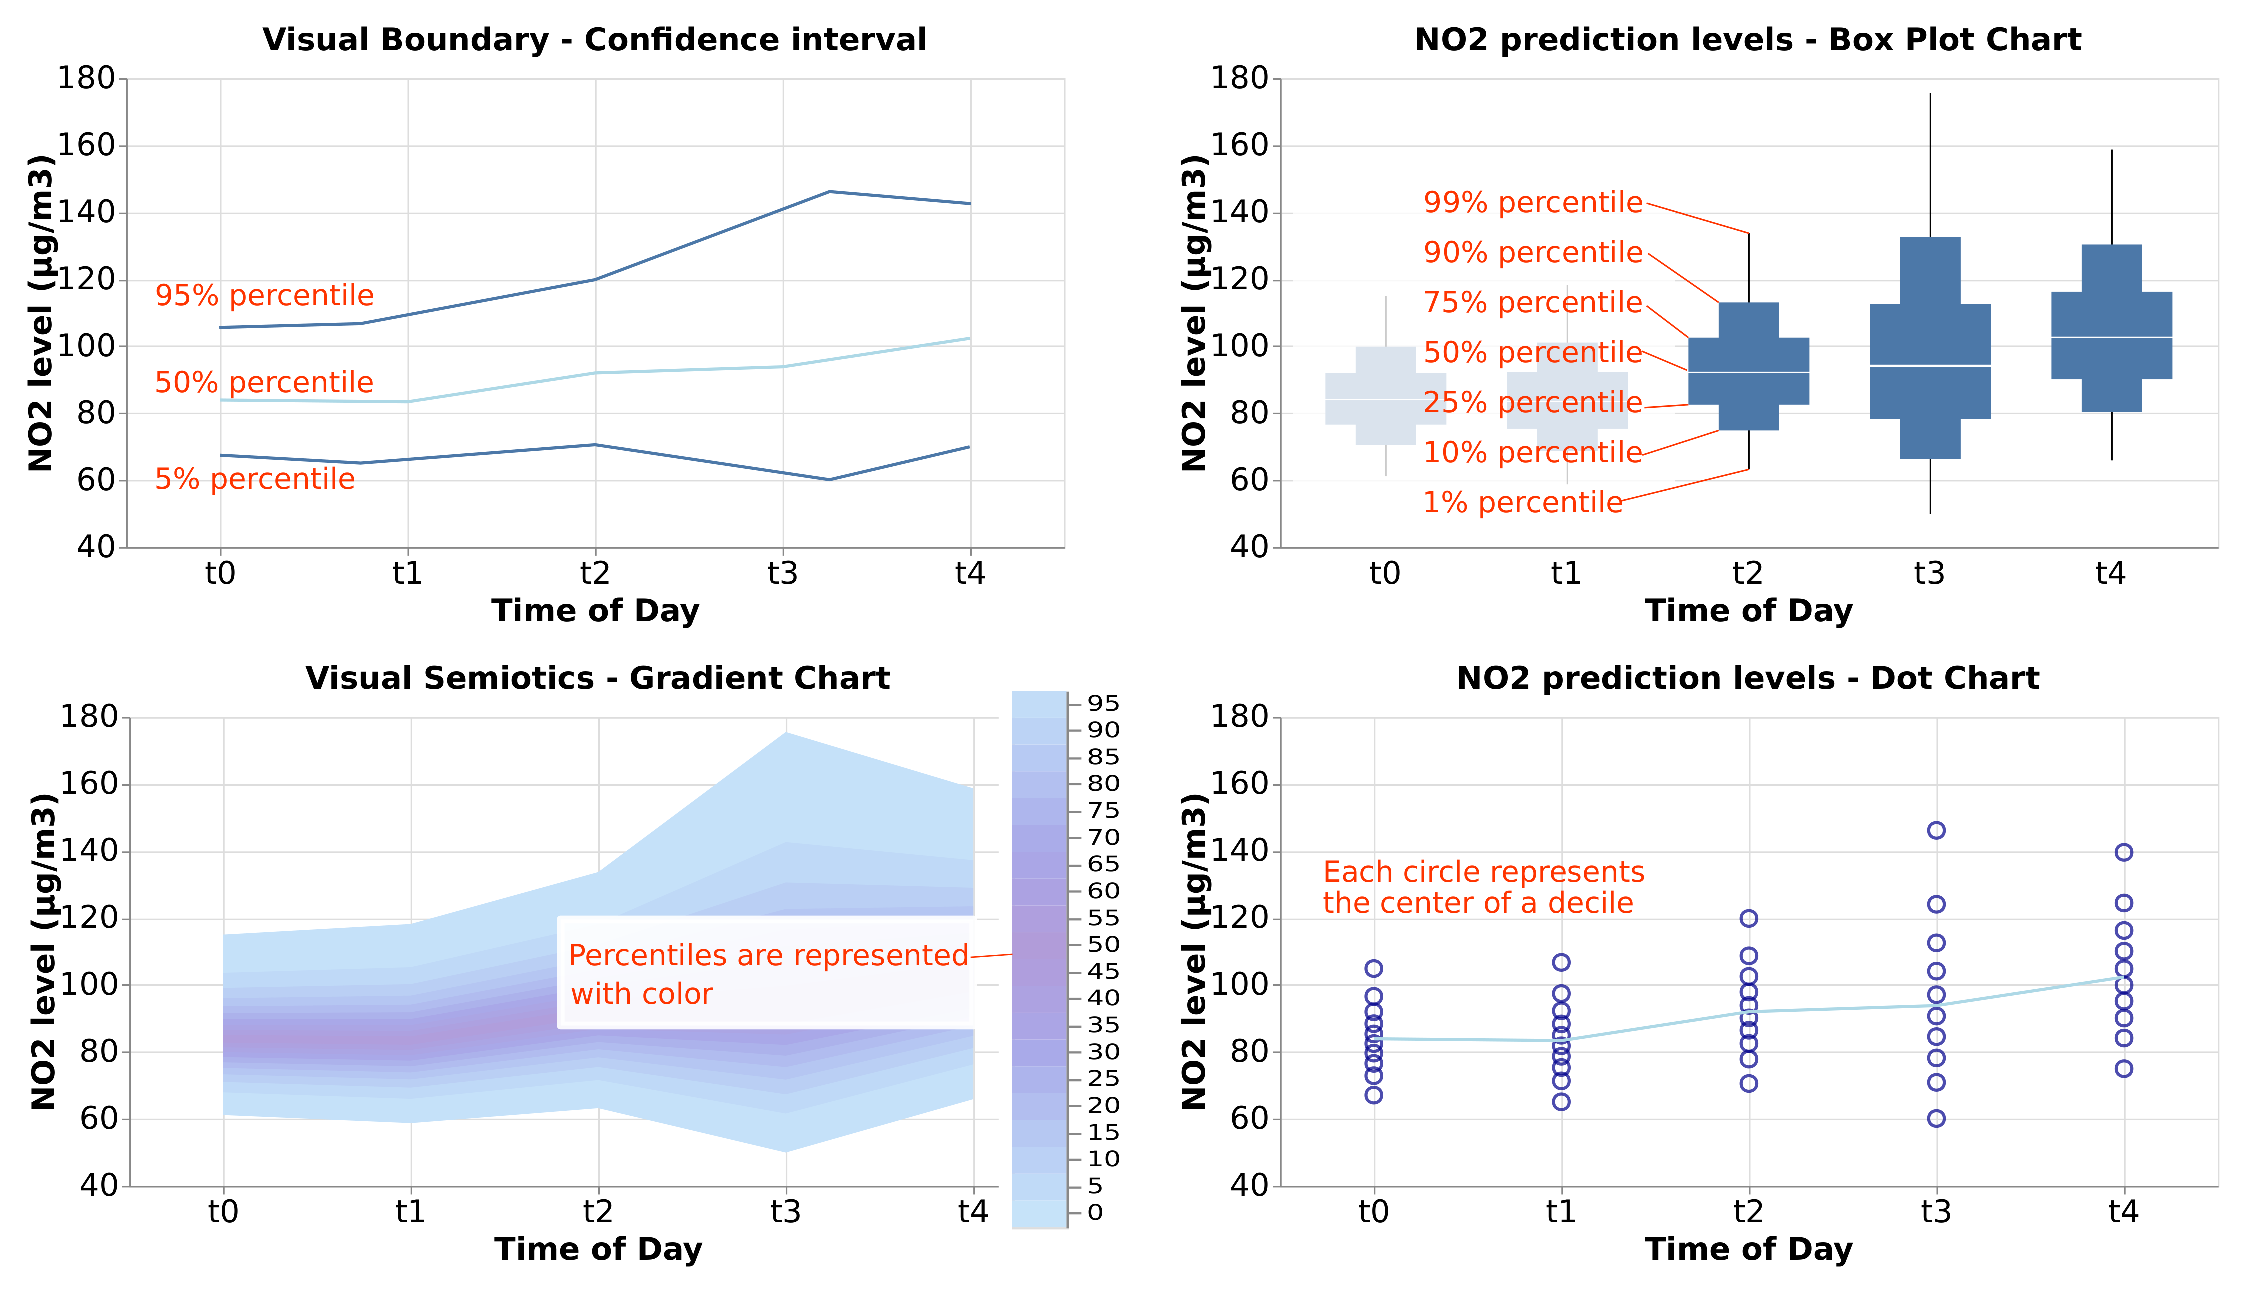
\includegraphics[width=.8\textwidth]{charts_vector} 
  \caption{\label{figure:charts} Probabilistic Forecast of NO2 levels in Madrid with different types of time Series Chart. 
  Top Left: Gradient Chart. Top Right: Box Plot. 
  Bottom Left: Confidence Interval. Bottom Right: Dot Chart.  }
\end{figure}

\section{Experimental Design}
\label{sec:exp_design}

We compare the readability of the four main types of probabilistic time series charts 
displayed in figure 1. We evaluate how well the charts can be read to estimate the probability 
that the evolving target is within a certain interval at a certain time point. As stated previously, 
the evolving distribution is the probabilistic forecast of NO levels. 

For this, we request the participation of users through the Amazon Mechanical Turk website. 
This service picks randomly 100 individuals with a minimum skill set (as proposed by Brenner 
et al., we select Master level participants, who are workers who 
''have consistently demonstrated a high degree of success in performing a wide range of HITs across a large number of Requesters'').

Each individual is presented a unique type of chart from the 4 presented above, gets a brief 
explanation on how it works and they have to estimate 5 probabilities from the chart. An example of
probability question is: "What is the probability of the NO2 levels being between 150 and 200 on 
November 21st at 22:00 ?". Individuals can provide their answers as a percentage or a 
decimal number between 0
and 1. We are also measuring the time it took to perform each estimation. 
As inspired by the work of Brenner et 
al. , once the individuals have estimated the probabilities, they are asked how confident they 
felt and how difficult the task was considered.

We are testing 20 individuals per type of chart and therefore we have 100 answers per 
type of chart.

\section{Results}
\label{sec:results}

First, we align all the answers in the same format: percentage, then for each answer, we define the 
reading error as the absolute value of the difference 
between the provided answer and the true probability displayed in the chart. Figure \ref{figure:errors} shows 
the distribution of the reading error per type of chart. We see clearly how the time series dot chart
has a much lower reading error then the other charts. 

\begin{figure}
  \centering
  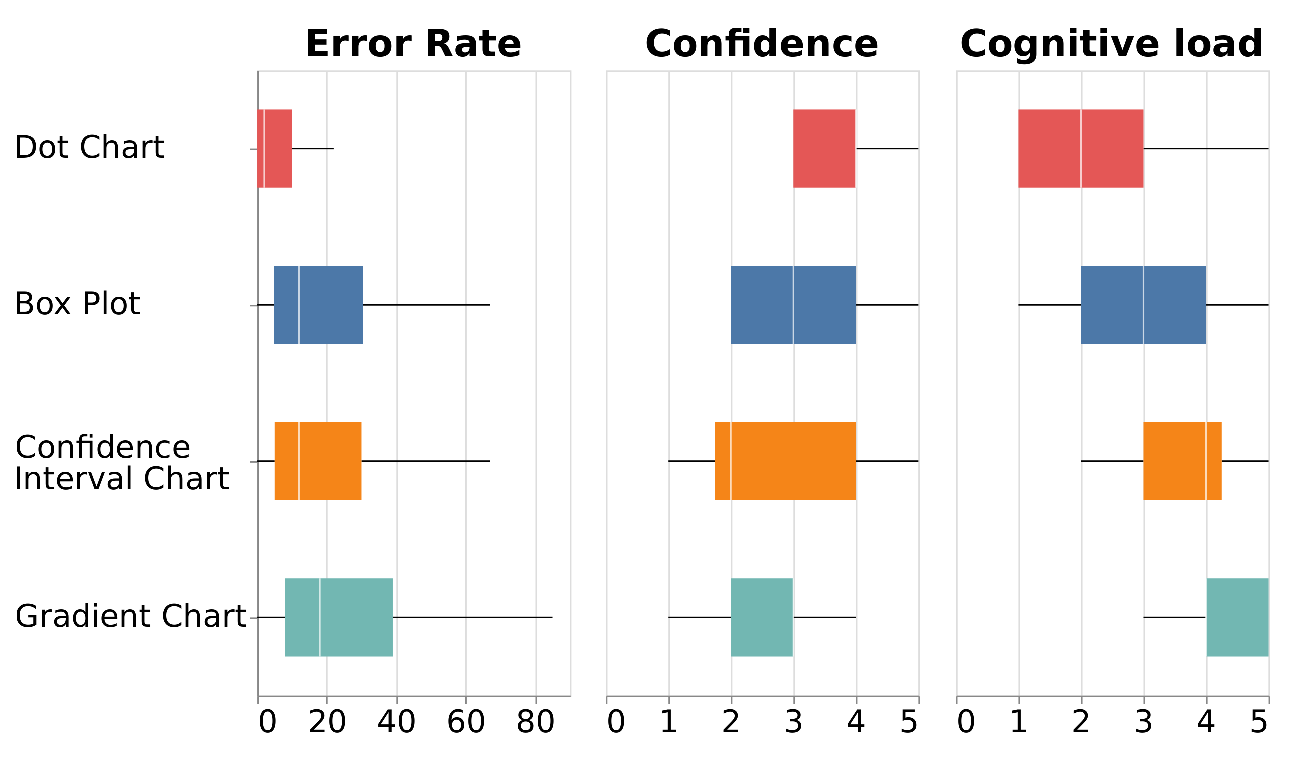
\includegraphics[width=0.9\textwidth]{comparison}
  \caption{\label{figure:errors}Error rate, confidence and cognitive load per type of visualization. 
  The whiskers represent the 10 and 90 percentile and the box shows the 25 and 75 percentile.}
\end{figure}

However, users does seem to need less time to answer the question as they were answering the questions. 
We see in figure \ref{figure:duration} that for every chart, the time it takes 
to read and answer the question decreases for every question answered. As we see in the figure, those times 
are very similar for all the types of charts. 

\begin{figure}
  \centering
   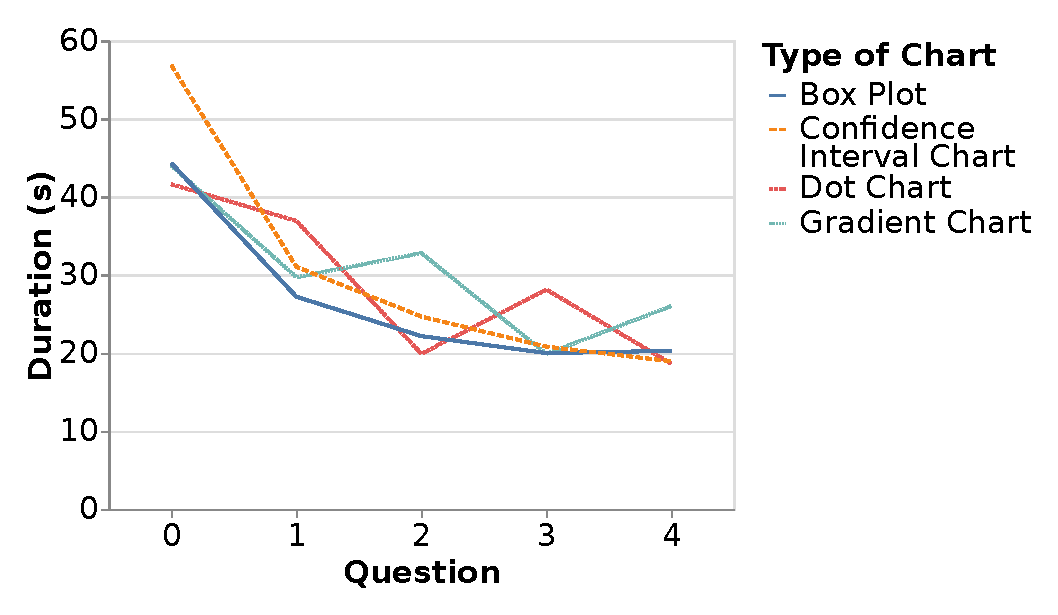
\includegraphics[width=0.6\textwidth]{duration_evo2}
  \caption{\label{figure:duration} Median Time it took to answer each question for each of the types of chart.}
\end{figure}  

Confidence and cognitive load charts (also shown on figure \ref{figure:errors}) also show the superior ease of use 
of the time series dot chart. Users reported higher levels of confidence and 
lower levels of cognitive load for the time series dot chart.


Finally although we selected users with master level, we still did received answers with probabilities 
above 1 or a probability as an interval. This could be due a lack of statistical knowledge from those 
users and reinforces the fears discussed in the introduction. 
We identified 9 users from 80 whose answers could not be used because of those reasons.

\section{Conclusions}
\label{sec:concl}

Although we could remark that the gradient chart, the box plot or the confidence interval charts are very good at 
providing an overall picture of the uncertainty in the time series, we can see from this work that the application of natural 
frequencies in an uncertainty chart does indeed
provide better numeric readability than any previous alternative. Natural frequencies does indeed simplify 
the statistic knowledge requirement and is also easier to read as it consists on counting.
We could improve even more the ease of use with interactive elements in the chart: for example
by applying different colors to the circles within a certain interval defined by the user interactively.

This type of chart is less well known that the other alternatives and an information effort should be made to motivate 
researchers and the general public to use it.




\section{References}
\label{sec:ref}


\bibliography{refs}

\end{document} 

